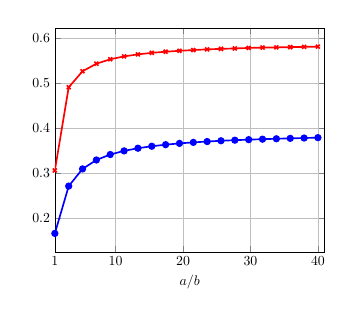
\begin{tikzpicture}[scale=0.5]
\begin{axis}[xlabel=$a/b$,ymajorgrids=true,xmajorgrids=true,xmin=1,xmax=41,xtick={1,10,20,30,40}]
%%%%%%%%%%% NATURAL CONFIGURATION
\addplot[Blue,mark=*,very thick] coordinates {(1.0,0.166671666717) (3.05263157895,0.271473241048) (5.10526315789,0.309586253757) (7.15789473684,0.329338030222) (9.21052631579,0.341437624903) (11.2631578947,0.349499284467) (13.3157894737,0.355401975072) (15.3684210526,0.359778334625) (17.4210526316,0.363232579694) (19.4736842105,0.366108924247) (21.5263157895,0.368318946347) (23.5789473684,0.370193175616) (25.6315789474,0.371917929706) (27.6842105263,0.373186889764) (29.7368421053,0.374390586011) (31.7894736842,0.375437438585) (33.8421052632,0.376327973806) (35.8947368421,0.377257456785) (37.9473684211,0.377959569069) (40.0,0.378803788038) };
%%%%%%%%%%% MODIFIED CONFIGURATION
\addplot[Red,mark=x,very thick] coordinates {(1.0,0.306123061231) (3.05263157895,0.490379640639) (5.10526315789,0.525847363737) (7.15789473684,0.542573846791) (9.21052631579,0.552360786766) (11.2631578947,0.558770850866) (13.3157894737,0.563263527372) (15.3684210526,0.566639350604) (17.4210526316,0.569151480988) (19.4736842105,0.571168869583) (21.5263157895,0.572820991368) (23.5789473684,0.574388901784) (25.6315789474,0.575434701715) (27.6842105263,0.576391027068) (29.7368421053,0.577495248637) (31.7894736842,0.578256308879) (33.8421052632,0.578705787058) (35.8947368421,0.5793468461) (37.9473684211,0.57984158789) (40.0,0.580405804058) };
\end{axis}
\end{tikzpicture}
%%% Local Variables:
%%% mode: latex
%%% TeX-master: "../../mainManuscript"
%%% End:
